\documentclass[conference]{IEEEtran}
\usepackage[utf8]{inputenc}

% correct bad hyphenation here
\hyphenation{op-tical net-works semi-conduc-tor}

\begin{document}

\title{En resa mot Svartåns djupa mörker}
\author{\IEEEauthorblockN{Felix Sjöqvist}
    \IEEEauthorblockA{MDH - School of innovation, Design and Technology\\
        Västerås, Sweden\\
        Email: fst17001@student.mdh.se}
\and
    \IEEEauthorblockN{Olle Olofsson}
    \IEEEauthorblockA{MDH - School of innovation, Design and Technology\\
        Västerås, Sweden\\
        Email: oon17003@student.mdh.se}
}

\maketitle
\section{Abstract}
\textbf{Boost converters is an important tool for many aplications including many small battery powered devices and hybrid electric vehicles. And for the engineer its function is of great importance. But so is it to be able to make one. This report explores the design and production of making a boost converter on a printed circuit board with the purpose to supply the reader with information about the experience that was gained doing this project. This includes what hardware and software was used, the choice of components, the manufactoring process and how the circuit finally got tested. The goal of the project was to successfully produce a working boost converter which actual measured voltage output is in pair with the simulated value. This is found to not be the case, possibly because of an unwanted short in the circuit.}


\section{Introduction}
\textit{Explain the subject. What was i studying? Why was this topic important to investigate? What did we know about the topic before I did this study? How will this study dvance new knowledge or new ways of understanding?}
\begin{itemize}
    \item Generally known information about the topic
    \item Prior studies' historical context to your research
    \item Your hypothesijks and overview of the results
    \item How the article is organized
\end{itemize}
\subsection{State of the Art}
\textit{The latest and most sophisticated or advanced stage of a technology or science. State of the art if the foundation for determining the methid and methodlogy.}
\subsection{Hypothesis}
\textit{In scienc, a hypothesis is an idea or explanation that you then tesr through study and experimentation. Outside science, a theory or quess can also be called a hypothesis}
\subsection{Research questions}
\textit{A research question guides and centers your research. It should be clear and focusd, as well as synthesize multiple sources to present your unque argument. RQ should be furmulat}

\section{Controlling output voltage}
The output voltage is controlled using the duty cycle of the input signal. The duty cycle is the fraction of the period in which the signal is active, and therefore takes on values between 0 and 1. A low duty cycle, say 0.25 will produce a low boost effect. This is because, the lower the time the mosfet is on i.e.\ letting current flow through it, the lower the time the inductor's magnetic field is charging up which boosts the output voltage during the signal off time. If the duty cycle instead were to be 0.75, the inductor would have a larger magnetic field to boost the output voltage. The theoretical output voltage can be expressed as the input voltage and the ducy cycle d:
\begin{equation}
    V_{out}=V_{in}/(1-d)
\end{equation}
The output voltage is also dependant on the frequency. Since there are inductive and capacative components in the circuit, the toal impedance is changing with the frequency. It is hard to know the actual total impedance of the circuit, and therefore finding an optimal frequency, but a good estimation of optimal frequency can be done by calculating the resonance frequency of the inductor and capatitor. This can be done using the following formula:
\begin{equation}
    f=1/(2\pi{}\sqrt{LC})
\end{equation}
In this case, with the components of this project, the resonance frequency is 5032Hz, which would make that a good starting point if one tried to maximize the voltage output.

\section{Hardware}
\begin{itemize}
        \item MyDAQ
        \item Voltera Printer
\end{itemize}

\section{Software}
Accompaning the earlier note on replicability, a similar description of suitable software substitutes will be provided, since the software choices relies heavily on the hardware used.\quad The only crucial software, if a setup similar to what was described above was to be used, would be the IDE used to program the Arduino board. One option is the official Arduino IDE, available as a web-based editor and as a desktop application\cite{arduino}.
\begin{itemize}
    \item Multisim\cite{multisim}, by National Instruments, was used to design and simulate the circuit, a software based environment allows for fast and easy experimentation, which is convenient in electronics design due to its trial-and-error nature.
    \item Ultiboard is another peice of software by National Instruments, with out-of-the-box integration with Multisim. It was used to design the actual PCB using the already-designed circuit from Multisim.
    \item Voltera for Windows 64-bit was used to interact with the Voltera printer.
\end{itemize}

\section{Choice of components}
The choice of componets was experimentally produced though the starting point were an erlier lab where a working boost converter was already designed. This design was of course not directly applicable to our project since this was not a surface mounted design. Different components were tested and simulated untill a desireble result was reached, see Tab~\ref{tab:comp}. Simulations were done using a $50\Omega$ resistor in series before the inductor to simulate a real inductor, which has a resistance. While small components often are desireble, the size can compromie circuit stability, espesially regarding capacitors. Therefore a smaller capacitor was not necessary.
\begin{table}[h]
    \begin{center}
        \caption{Choice of components}
        \label{tab:comp}
        \begin{tabular}{c|c|c|c}
            Component & Name & Value & Footprint (\%)\\
            \hline
            Capacitor & - & 1uF & CAPC2012X145N\\
            Inductor & - & 1mH & INDC4520X140N\\
            MOSFET & 2N7002K & - & SOT95P230X110-3N\\
            Diode & D1N4148 & - & SOD2513X110AN\\
            Resistor & 5000 & 4700\Omega$ & RESC1608X63N\\
            Pin strip & Pin strip & 2x7 & Custom\\
        \end{tabular}
    \end{center}
\end{table}

\section{Manufacture Process}
This section will describe the full process of developing the step up converter PCB\@. That is simulation, PCB layout, and printing.\
\subsection{Design and simulation}
Firstly, simulations were made to experimentally come up with a theoretical solution to the problem. In this stage, total freedom was at hand which made the ability of finding errors and differentiate good solutions from bad ones simpler. The simulations were made in Multisim using the build in function generator and multimeter to measure the outcome. When the desired function had been simulated and verifired, the netlist, which is a description of the connectivity of the circuit, was carefully verified to maintain the desired function going into Ultiboard.
\subsection{PCB layout}
The Multisim file was transfered to Ultiboard where the last design choices were to be made. In Ultiboard, two crucial files were constructed.

The first one \textit{''Copper Top''}, which contains the information of where the printer shall print the silver traces, connecting all the components. Thanks to the netlist from Multisim, Ultiboard automatically connects all components making the process significantly easier. The components were placed as compact as possible, with simplicity in mind, see Fig.\ref{fig:PCB}. Next trace width and trace clearence was chosen to handle the voltage, current and frequency the circuit was designed for.

The next file \textit{''Solder Mask Top''}, contains information about where the printer shall print the soldering masks that the physical components later can be placed and soldered on to. This information is automatically generated from the footprints of the components, being chosen in the Multisim file.
\subsection{Printing}
After connecting the Voltera printer to the computer, the gerber file \textit{''Copper Top''} form Ultiboard was exported to the Voltera software to begin the printing process. The conductive ink \textit{''LaughingBear''} was used as the conductive trace material. The printer flow was calibrated to ensure good quality traces and pads with neither too much flow, resulting in possible shorts, nor too less, resulting in possible broken traces. The traces were printed and inspected to watch for possible faults. The board was then baked for about 30 minutes, using the ink specific, Voltera baking program, to harden the printed silver ink.

After the baking, the next gerber file \textit{''Solder Mask Top''} was loaded to begin the second printing phase. Here, the solder paste \textit{''FuriousAnt''} was used for the solder masks. The solder masks were printed and inspected to watch for possible shorts.

With solder paste on the pads, the components were ready to be placed on the board. A Small amount of extra solder paste was manually put on the pads of the pin strip footprint to strengthen the otherwise delicate structure. All the components exept the pin strip were carefully placed on the board using the component placing machine. The pin strip was manually placed on the board. Then the board was reflow soldered using the Voltera reflow program, this again took about 30 minutes.
\begin{figure}[h]
    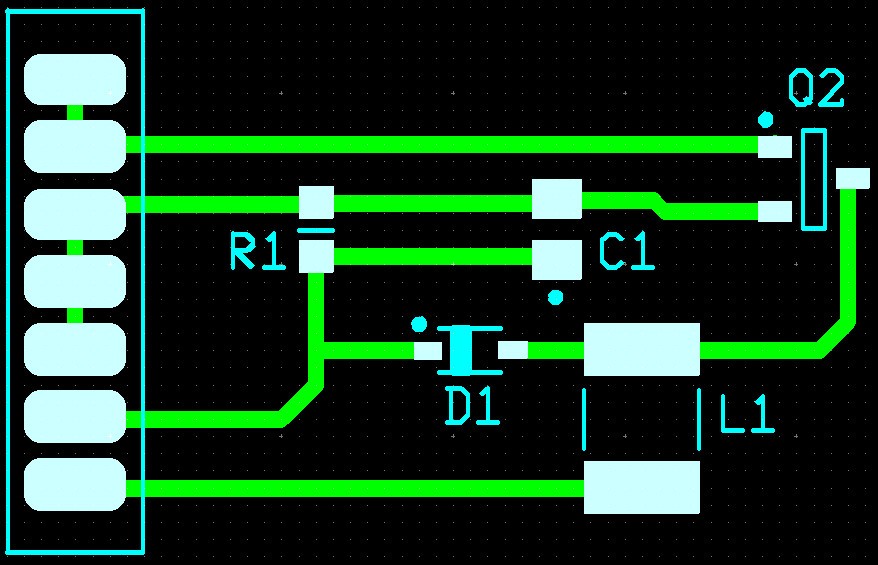
\includegraphics[width=\linewidth]{PCBlayout.jpg}
    \caption{Picture of the layout of the components on the PCB\@. R1\hyp{}resitor, D1\hyp{}diode, C1\hyp{}capacitor, L1\hyp{}inductor, Q2\hyp{}mosfet.}
    \label{fig:PCB}
\end{figure}

\section{Method}
\subsection{Problem formulation}
ja det verkar som att problemformuleringen ska vara här
\textit{The problm formulation is defined upon hypothesis to define the problem or problems for the thesis}
\textit{How will you test the hypothesis? What methods will be used from the knowledge learned in state of the art?}
\\The PCB was tested using the National Instruments myDAQ, by powering the PCB with the myDAQ:s constant 5V output and then imposing a square wave on the input pin with following characteristics:
\begin{itemize}
        \item Constant 5V amplitude.
        \item Constant 2.5V positive offset.
        \item Variable frequency $100Hz-10kHz$
        \item Variable duty-cycle $10\% - 90\%$
\end{itemize}
The voltage across GND and Output was measured whilst modifying the variables above, see \ref{fig:pcb} for more details.
\begin{figure}
    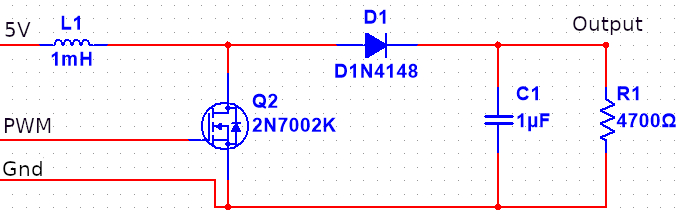
\includegraphics[width=\linewidth]{CircuitDesign.jpg}
    \caption{Multisim diagram of the circuit used in this report}
    \label{fig:pcb}
\end{figure}


\section{Results}
The technuiqe outlined above generated the rusults in \ref{tab:meas}.
\begin{table}[h]
    \begin{center}
        \caption{Step-up output voltage with varying frequency and duty cycle}
        \label{tab:meas}
        \begin{tabular}{c|c|c}
            $V_{out}$ & Freq. (\textit{Hz}) & Duty cyc. (\%)\\
            \hline
            4.87 & 100 & 10\\
            4.88 & 100 & 50\\
            4.87 & 100 & 90\\
            4.87 & 5000 & 10\\
            4.86 & 5000 & 50\\
            4.85 & 5000 & 90\\
            4.87 & 10 000 & 10\\
            4.88 & 10 000 & 50\\
            4.89 & 10 000 & 90\\
        \end{tabular}
    \end{center}
\end{table}

\section{Conclusion}
As evidenced by the results above, our method did not produce the predicted results of $~25V$ at $10 000Hz$ and $90\%$ duty-cycle.

\section{Discussion}
Since the method outlined in this paper did not produce the predicted results and our hypothesis hence remains unproven, a deeper discussion of the apparant failure is of high interest. A correlation between $V_{in} = 5V$ and $V_{out} \approx 5V$ was quickly made, leading to the assumption that some sort of short between $V_{in}$ and $V_{out}$ had occured, the investigation ensued. The thick layer of (non-conducting!) hot-glue, earlier applied as a mechanical safety procedure after repeated pin header related failures, was carefully removed using a flat head screwdriver and rigorus amounts of determination. On closer inspection of the PCB, a short between $V_{in}$ and $V_{out}$ was observed, see Fig.\ref{fig:short}

\begin{figure}
    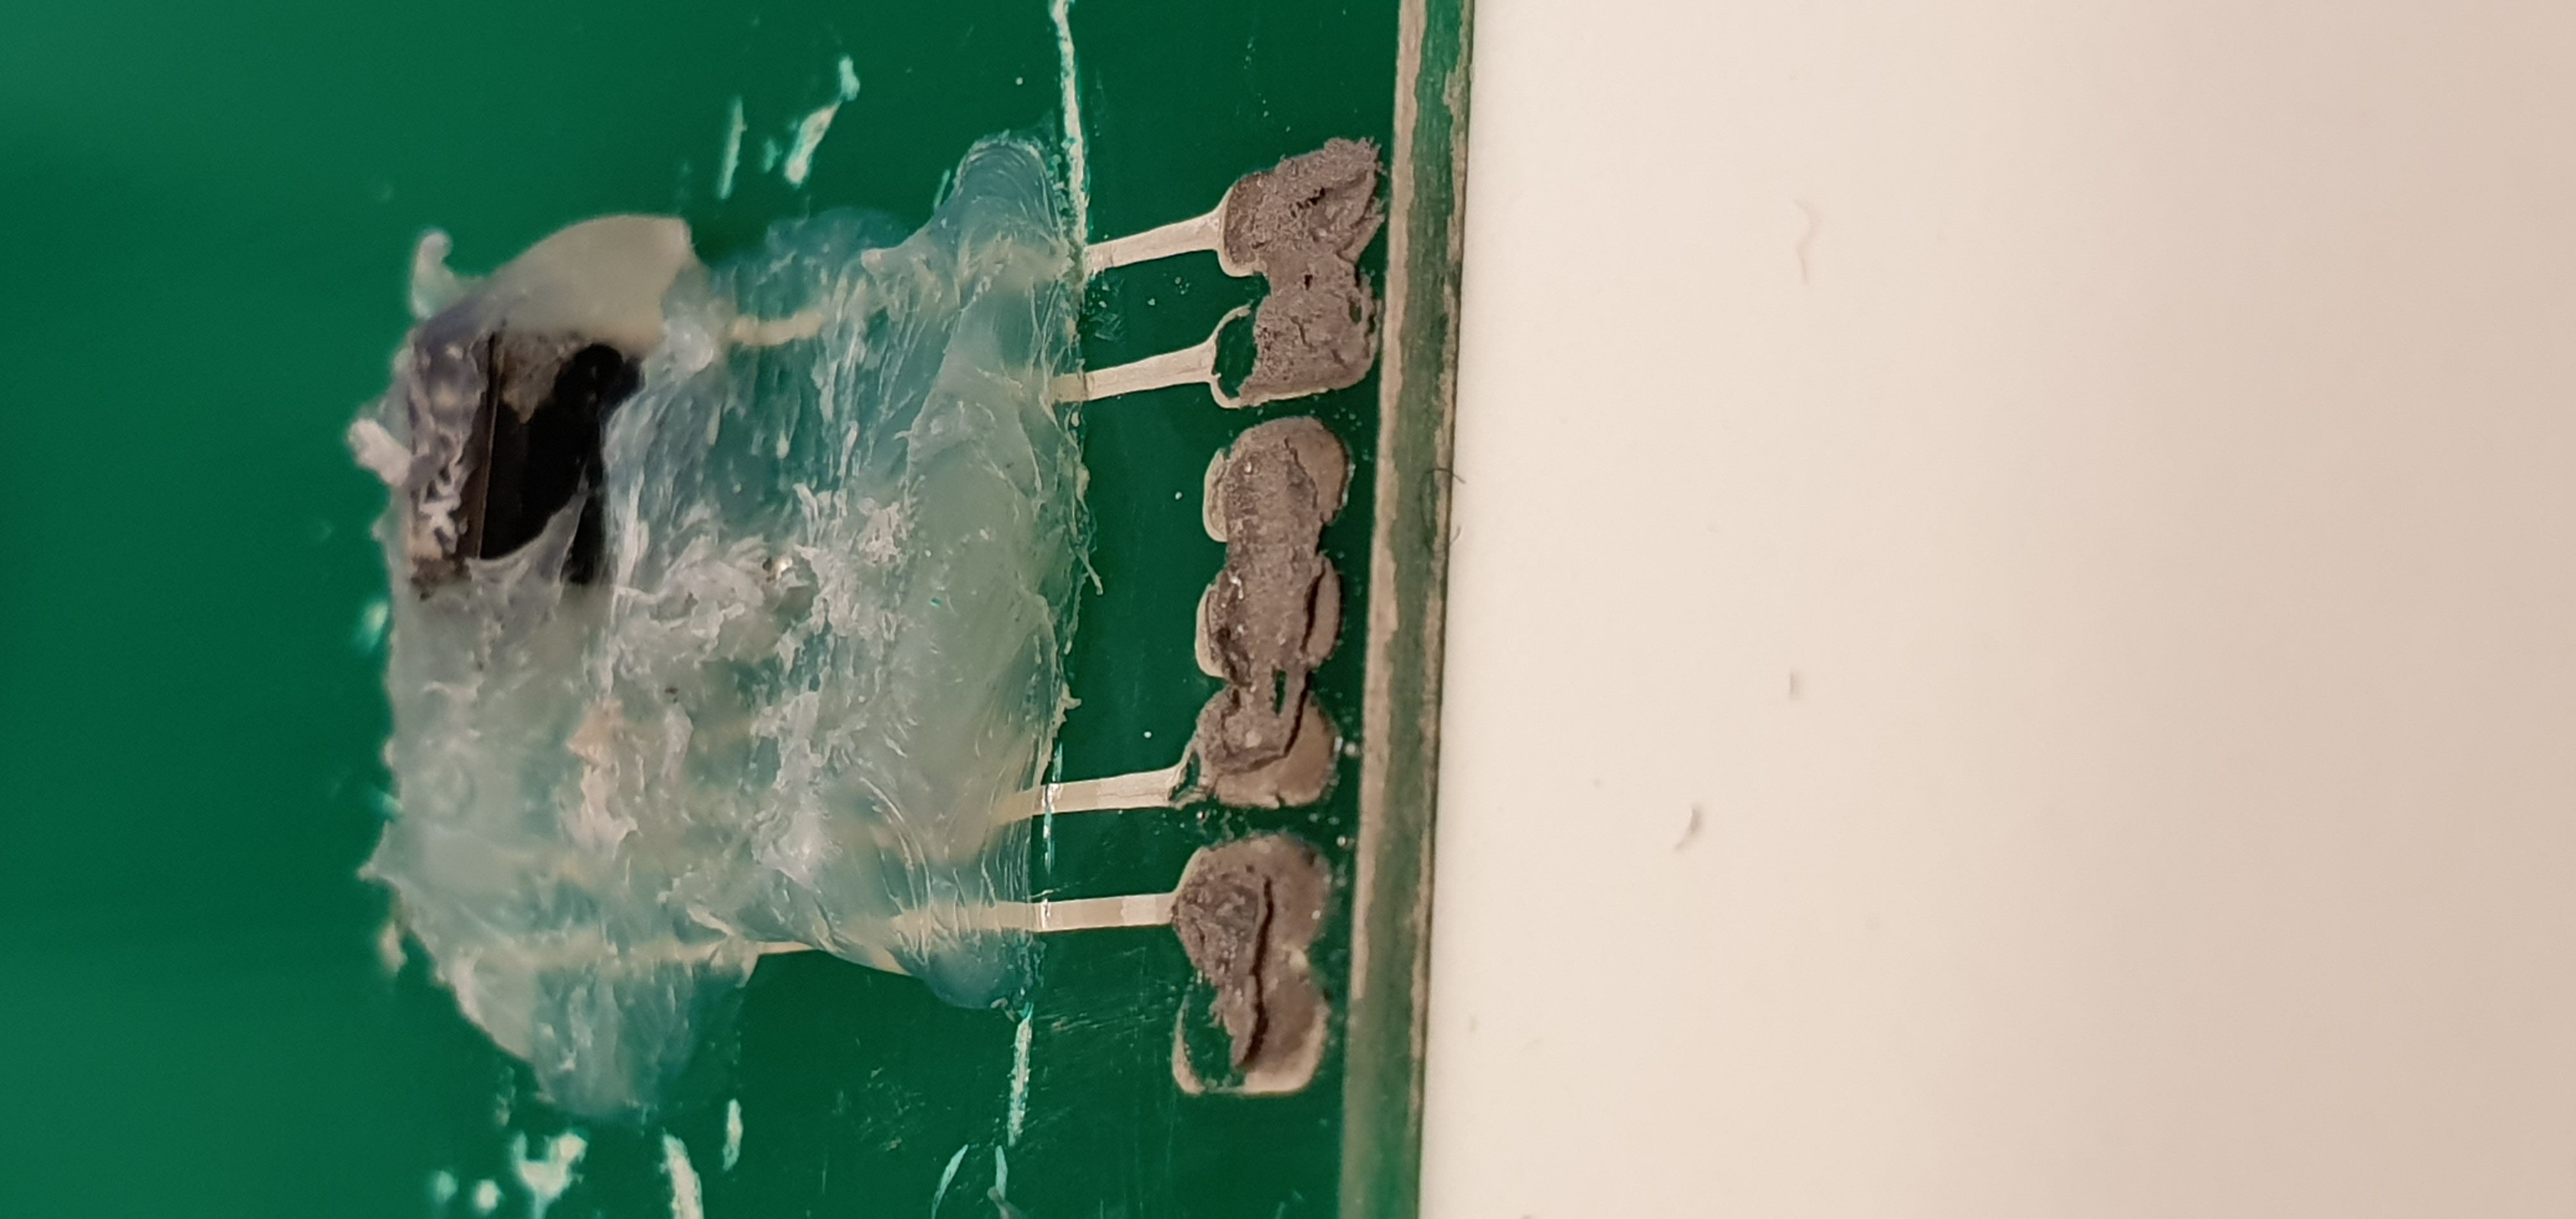
\includegraphics[width=\linewidth]{ela302-kortslutning.jpg}
    \caption{Picture of a short on the pin header.}
    \label{fig:short}
\end{figure}


\begin{thebibliography}{1}
\bibitem{IEEEhowto:kopka}
H.~Kopka and P.~W. Daly, \emph{A Guide to \LaTeX}, 3rd~ed.\hskip 1em plus
  0.5em minus 0.4em\relax Harlow, England: Addison-Wesley, 1999.
\end{thebibliography}

\end{document}


